\documentclass{article}
\usepackage[utf8]{inputenc}
\usepackage{amsmath,amsthm,amssymb}

\title{Solution Mannual for Supplyment Psets of MIT OCW 18.02SC Fall 2010}
\author{Lu YuXun}
\date{February 2017}

\usepackage{natbib}
\usepackage{graphicx}

\begin{document}

\maketitle

\section{Psets 1}
\subsection{1. Vectors and Matrices}
\textbf{1A-12*} Label the four vertices of a parallelogram in counterclockwise order as OPQR. Prove that the line segment from O to the midpoint of PQ intersects the diagonal PR in a point X that is 1/3 of the way from P to R.
\begin{figure}[htp!]
    \centering
    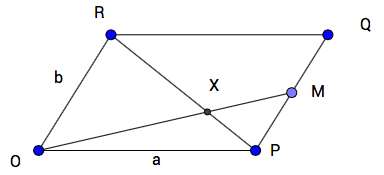
\includegraphics[width=50mm,scale=0.5]{Figure/1A-12.png}
    \caption{1A-12 Figure}
    \label{1A-12 Figure}
\end{figure}
\begin{proof}
Suppose $\overrightarrow{OP} = \mathbf{a}$ and $\overrightarrow{OR} = \mathbf{b}$.
\\ We have: $\overrightarrow{RP} = \mathbf{a} - \mathbf{b}$ (1), $\overrightarrow{OM} = \mathbf{a} + \frac{1}{2} \mathbf{b}$ (2), $\overrightarrow{OX} = \mathbf{b} + \overrightarrow{RX}$ (3).
\\Let $\overrightarrow{OX} = u(\mathbf{a} + \frac{1}{2}\mathbf{b})$, $\overrightarrow{RX} = (1 - v)(\mathbf{a} - \mathbf{b})$.
\\ From (3) we can derive:
\\ $\mathbf{b} + \overrightarrow{RX} = \overrightarrow{OX} = u\mathbf{a} + \frac{u}{2}\mathbf{b} = \mathbf{b} + (1-v)\mathbf{a} - (1-v)\mathbf{b}$
that is, 
\begin{equation}
    \begin{cases}
    u = 1 - v
    \\ v = \frac{u}{2}
    \end{cases}
\end{equation}
Solve equations in (1), we have $u = \frac{2}{3}, v = \frac{1}{3}$. So $\overrightarrow{OX} = \frac{2}{3} \overrightarrow{OM}$ and $\overrightarrow{RX} = \frac{2}{3} \overrightarrow{RP}$, i.e. the intersection point X of RP and OM is 1/3 of the way from P to R.
\end{proof}

\end{document}
